\documentclass[conference]{IEEEtran}
\usepackage{algorithm}
\usepackage{algorithmic}
\usepackage{graphicx}
\usepackage{subfigure}
\usepackage{float}
\usepackage{amssymb}
\usepackage{amsmath}
\usepackage{textcomp}

\IEEEoverridecommandlockouts    
\textwidth 178mm    
\textheight 239mm  
\oddsidemargin -7mm
\evensidemargin -7mm
\topmargin -6mm
\columnsep 5mm

% todo
\usepackage{color}
\newcommand{\todo}[1]{\textcolor{red}{\texttt{#1}}}

\begin{document}
\title{\ \\ \LARGE\bf Off-line cursive handwritten word recognition using hidden Markov models}
\author{{\bf Davide Modolo} and {\bf Thijs Kooi}\\ dmodolo@student.uva.nl, Thijs.Kooi@student.uva.nl}
\maketitle
\begin{abstract}
Over the past decades, much research has been performed in the field of optical character recognition and where the research in recognizing typewritten words and handwritten isolated characters has given rise to a variety of robust methods, the recognition of cursive handwritten words remains a challenge.
%This paper describes a complete system for the recognition of off-line handwriting. Preprocessing techniques are described, including segmentation and normalization of word images to give invariance to scale, slant, slope, and stroke thickness. Representation of the image is discussed and the skeleton and stroke features used are described.

 In this paper we explore different aspects of off-line handwriting recognition, a task that does not furnish temporal information, and apply a hidden Markov model to estimate probabilities. We apply the method to some simple word recognition tasks and subsequently use a larger dictionary to see how the system performs in a more realistic setting. Results show...
\end{abstract}
\section{Introduction}
Even though contemporary communication seems to emphasize on electronic information exchange rather than pen and paper, we still encounter cursive reading and writing on a daily basis. In the pursuit of making our lives easier, computers may serve a purpose by mitigating laborious document transcription. For applications one can think of tasks such as automatically processing bank checks, various application forms and address lines on an envelope.

The field of optical character recognition (OCR) is a sub field of pattern recognition and computer vision and is concerned with this automatic casting of analog character sequences to a digital mould. The area can be dichotomized into typewritten and handwritten character transcription, with the latter further split into on-line and off-line recognition. In the case of on-line recognition, the path of the pen is followed, thereby providing efficacious data about the nature of the character and the technique can be applied in devices that make use of a touch screen of some kind. On the other hand, off-line handwritten word recognition does not incorporate the temporal dimension, rendering it harder but consequently more widely applicable. Despite ongoing academic attention, and the availability of successful commercial systems for typewritten and isolated characters, cursive character recognition remains a formidable challenge. 

Over the past decades, researchers have performed in-depth studies of different fields of the recognition pipeline, however, no consensus has been reached as to what is the most effective method at each stage. The overall routine however, seems to follow the same pattern. In the first stage, the image of the word or document is pre-processed and typically normalized. The second stage generally involves feature extraction, followed by the use of some pattern recognition technique. Although many methods make us of a hidden Markov model (HMM) \cite{journals/ijprai/MartiB01,journals/pr/BunkeRS95} to parametrize the character or word distributions, alternatives have been researched. Artificial neural networks (ANN) are commonly combined with the HMM \cite{journals/pami/GravesLFBBS09} to model, for example, the probability of a character, given a certain observation. Schomaker \cite{bb105728}, applies an ANN in the form of a Kohonen self-organizing map to model cursive script. An extended mean shift clustering method has proved to be successful in clustering Japanese characters in a high-dimensional space \cite{bb105468}. Instead of statistical modeling a form of edit distance was used by Park and Govindaraju \cite{CVPR00_VOLII*290} to characterize words.

Apart from character and word classification, an OCR system can also focus on writer identification \cite{bb106176, oai:oai.columbia.edu:epic/nsdl/1/145780}, which has applications in forensic science and to identify users of a system. Instead of normalizing writer variations, as we would in recognition tasks, the key idea is now to focus on salient writer-specific traits.

In this paper we will take a bird eye view of the whole OCR pipeline, without overly scrutinizing specific stages. The typical OCR pipeline has different stages: pre-processing, feature extraction and classification, and it is shown in Fig. \ref{fig:pipeline}. We will apply different pre-processing methods to segment sentences and words and normalize the characters. Rudimentary features will subsequently be extracted from the acquired images and we will use a sliding window to obtain observation sequences. To classify the words, we will make use of the HMM and will experiment with different parameters and observation distributions in the attempt to optimize recognition performance. The methods will first be tested on simple recognition tasks and subsequently in a more realistic setting with a larger dictionary.

\begin{figure}[H]
 \centering
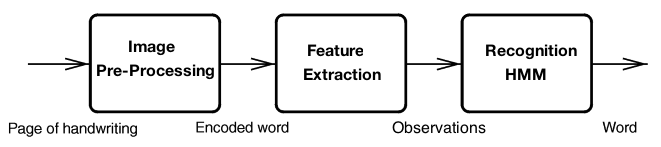
\includegraphics[width=0.55\textwidth]{pipeline.png}
\caption{A schematic of the recognition system.}
\label{fig:pipeline}
\end{figure}

This paper is divided into 5 sections, with each section covering a different aspect of the pipeline. In Sec. 2, we will describe this pipeline along the  pre-processing methods used. Sec. 3 will cover feature extraction, followed by a brief overview of the HMM paradigm. In Sec. 4, the experimental setup will be discussed, along with the results acquired and we will end with a conclusion and discussion in Sec. 5.

\section{Preprocessing} \label{sectP}
Several general preprocessing steps are done on the composite raw image before word recognition starts. These steps attempt to normalize the image as much as possible. It is assumed that the image has been binarized from gray scale. 
A pipeline of the preprocessing is shown in Fig. \ref{fig:pipelinePP}, and in the next subsections we will briefly describe all the steps involved. It is worth to note that in the presented pipeline skew and slant correction steps are applied both to lines and individual words. The repetition is useful to first obtain a good word segmentation, and to then obtain a good estimation of the baselines on single words.

\begin{figure}[H]
 \centering
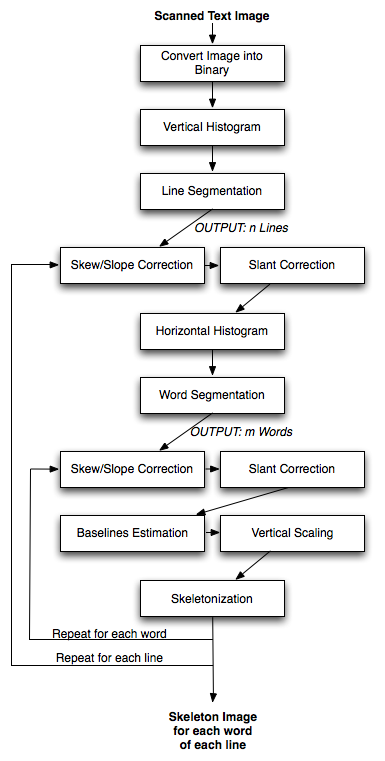
\includegraphics[width=0.45\textwidth]{preprocessing_pipeline.png}
\caption{Our pipeline of the preprocessing part of the system.}
\label{fig:pipelinePP}
\end{figure}
 

\subsection{Line Segmentation}
Line segmentation is used to divide text of document into individual lines for further preprocessing. Line segmentation works on the assumption that the lines of the text are relatively horizontal. First, a histogram of black pixels of the image in the \textit{y} direction is generated and smoothed with a median filter, where median filtering is used to remove insignificant minima and maxima; and then, cuts are made at significant local minima (often 0).

\subsection{Skew Correction}
The skew correction procedure rotates the text line such that the line on which the words are written becomes horizontal. For this purpose two steps are applied. First, the skew angle is estimated. Second, the input image is rotated by the estimated skew angle. 
To estimate the skew the lowest black pixel in every column are determined, and the set P defined as:
\begin{equation}
P = \{p_i = (x_i, y_i) | \text{lowest black pixel in column } x_i\}
\end{equation}
is populated.
Once $P$ has been populated, a least-squares linear regression is computed to find a line on the form $y = ax + b$ to fit as baseline of the input line. Then, the rotation angle is computed as $\theta = \arctan(a)$, as the image is rotated by $- \theta$ to remove the skew.


\subsection{Slant Correction}
The goal of slant correction is to bring the handwriting into an upright position. Depending on the writing style, the handwriting (especially its long vertical strokes) is more or less slanted to the right or to the left. Similar to the skew correction, two steps are applied to remove the slant. First, the slant angle is estimated from the image. Second, an affine transformation with the estimated slant angle brings the handwriting into an upright position.
The slant is estimated by finding the average angle of near-vertical strokes.  First, the contour of the thresholded image is found, and a chain of connected pixels representing the edges of stroke is obtained. Second, the mode orientation of those edges close to the vertical is used as overall slant estimate.  


\subsection{Word Segmentation}
Word segmentation is used to split lines into individual words, again, for further preprocessing. 
Word segmentation is not always straight-forward. Gaps between words are generally expected to be larger than gaps between characters in a word. This however, is not necessarily true. Variations are ordinary and ligatures and flourish often cause larger geometric gaps to appear small, resulting in improper word segmentation \cite{springerlink:10.1007/s100320050035}. A neural network could be used to intelligently segment words, but in our implementation we used a slightly less robust, but significantly faster approach. First, all the white spaces in \textit{y} direction in the line are estimated, where a white space is defined as one or more (consecutive) columns of zero black pixels. Then, k-means clustering is performed on the white spaces with $k=2$ to separate significant divisions (white spaces between words) from insignificant divisions (white spaces between characters).
 

\subsection{Baselines Estimation}
Four horizontal lines (ascender, upper, lower and descender - ordered from the top to the bottom) must be fit to the line of text for proper scaling and, later, recognition. 
Determining the upper and lower baselines is rather trivial, and can be done using linear regression as explained in skew subsection. Upper black pixels of each column are used to determine the upper baseline, and lower black pixels are used to determine the lower baselines. 
Ascender and descender baselines can be estimated respectively as the first $y$ non-zero value and the last $y$ non-zero value on the vertical histogram of the line. 
Once the baselines are estimated the input line can be horizontally divided into three parts, the descender part, the middle part, where the body of the text is located, and the ascender part.  The rest of the image (above the ascender baseline and below the descender baseline) is discarded. 

\subsection{Vertical Scaling}
In this step, the three regions defined in the previous subsection, are scaled to a predefined height. This normalization makes the feature extraction more robust because the location of the handwriting is correlated to the corresponding characters. Some characters, e.g. �a� or �e�, are entirely written in the middle part, whereas uppercase letters and characters like �l� and �t� also involve the ascender part.

\subsection{Skeletonization}
Before passing the image to the recognition system, the image has to become a skeleton.
The image is first smoothed by convolution with a 2-dimensional Gaussian filter to remove noise and to correct some handwritten mistakes (e.g. the bottom loop of the letter g is not complete and it misses few pixels). Next, an iterative, erosive, thinning algorithm is applied to reduce the stroked in the writing to the width of a pixel. The obtaining image is called the skeleton of the word. 

\section{Feature extraction}
After preprocessing, a feature extraction method is applied to capture the most relevant characteristic of the word to recognize.
As in most machine learning and pattern recognition tasks, feature extraction is of vital importance; a highly complex recognition model will yield poor results if features are not selected properly. In this stage, we try to look for the aspects of the data that are most informative of the class.\\
All the features are extracted from the skeleton of the image obtained after the preprocessing step of the pipeline. 
In our implementation we mainly focused on two types of features: statistical and morphological. \\
The former only represent low-level information about the word, and they are based on the percentage of black pixels in the three regions of the word: ascender, middle and descender, respectively.\\
The latter represent salient information about the word. They are often more discriminative, and they have been found to reduce the error rate significantly \cite{10.1109/34.667887}. Those features are:
\begin{itemize}
\item {\bf Dots}: Dots above the letters 'i' and 'j' can be identified as short, isolated strokes occurring in the ascender part of the word.
\item {\bf Junctions}: Junctions occur where two stroked meet or cross and are easily found in the skeleton as points with more than two neighbors.
\item {\bf Endpoints}: Endpoints are points in the skeleton with only one neighbor and they mark the ends of strokes. 
\item {\bf Loops}: Loops are found from connected-component analysis on the skeleton, to find areas of background color not connected to the region surrounding the word. 
\end{itemize}

\begin{figure}
 \centering
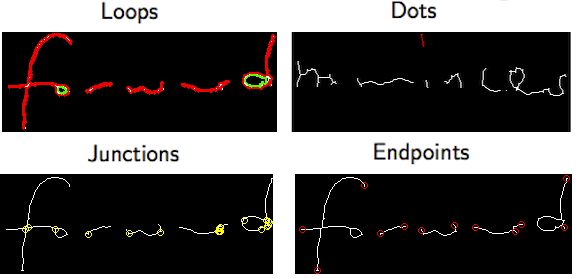
\includegraphics[width=0.47\textwidth]{features2.png}
\caption{Example of morphological features.}
\label{fig:pipeline}
\end{figure}

For a word, each of the features above could be encoded as a single number, the total number of occurrences, but as it is useful to know whether i.e. a loop or a dot is present in a particular frame, the positions of the dots, junctions, endpoints and loops are also stored. \\



\todo{new paragraph ? }
In order to exploit the sequential nature of the observations, we need a model that does not treat the data as i.i.d. This is provided by the {\it hidden Markov model} (HMM) \cite{rabiner-89,Rabiner86Z27}, a generative classifier, widely applied in areas such as speech and gesture recognition and computational linguistics.


\section{Hidden Markov models}
The HMM can be understood from different perspectives. It bears strong resemblance to the finite state automaton and can essentially be seen as a specific type of graphical model. Moreover, researcher acquainted with the POMDP formalism will see familiar aspects. An HMM can be formally described by:
\begin{itemize}
 \item A set of $N$ states $S = (s_{1}, s_{2}, \ldots, s_{N})$, where the state of the system at time $t$ is denoted $q_{t}$
 \item A set of priors ${\bf \pi} = (\pi_{1}, \pi_{2}, \ldots, \pi_{N})$, providing the probability $P(q_{1} = s_{i})$.
 \item A transition function ${\bf A}$, where $a_{ij} = P(q_{t+1} = s_{j} | q_{t} = s_{i})$. 
 \item An observation function ${\bf B}$, mapping each observation at every state to a probability $b_{i}({\bf o}_{t}) = P({\bf o}_{t} | q_{t} = s_{i}, \lambda)$, where $\lambda$ denotes the model parameters.
\end{itemize}
The model is trained to estimate the posterior probability $P({\bf O}|\lambda)$ of an observation sequence ${\bf O} = ({\bf o}_{1}, {\bf o}_{2}, \ldots, {\bf o}_{T})$, with $D$-dimensional observation vectors ${\bf o}_{t} = (o_{1},o_{2},\ldots,o_{D})$. We assume time to be discrete and the transition and observation probabilities to be static. The hyper parameters we have to concern ourselves with are the network topology, i.e., the number of states and the transition probability and choice of the observation or emission probability function. In general, the exact state sequence remains hidden, hence the name {\it hidden} Markov model. The Markov property describes the dependency relation between subsequent data points. For speech and handwriting recognition a left-to-right model is generally applied, as show in figure 1, though variations exist.\\
\begin{figure}[H]
 \centering
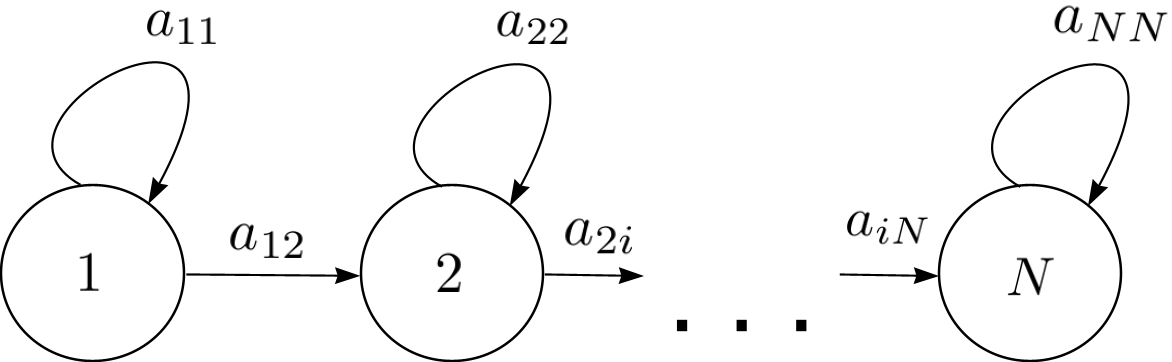
\includegraphics[width=0.4\textwidth]{hmm.jpg}
\caption{Illustration of a simple left-to-right model}
\end{figure}
The three main problems to be solved for this model architecture are:
\begin{enumerate}
 \item The probability of an observation sequence, given the model, $P({\bf O}|\lambda)$.
 \item The most likely state sequence, underlying a given observation sequence and the model, $Q^* = \max P(Q|{\bf O},\lambda)$.
 \item The most likely parameters of the model $\lambda^* = \max P(X|\lambda)$, given a training set of $M$ observation sequences $X = ({\bf O}_{1}, {\bf O}_{2}, \ldots, {\bf O}_{M} )$.
\end{enumerate}
The third problem is solved by the Viterbi algorithm, but will not be needed for out particular task. A naive way to address the first problem of estimating the posterior probability of an observation sequence, would be to simply marginalise over all possible state sequences ${\bf Q}$ and evaluate their probability. Unfortunately, the cardinality of ${\bf Q}$ increases exponentially with the number of observations, rendering the method $\mathcal{O}(N^{T})$ and thereby infeasible for all but the smallest models. Luckily, an alternative exists in the form of the {\it forward-backward} algorithm, a special instance of the {\it sum-product} algorithm.
\subsection{Forward-backward algorithm}
The forward-backward algorithm is an efficient way of computing the probability of an observation sequence, given the model. The forward probability, is defined as the probability of a partial observation sequence ${\bf o}_1, {\bf o}_2, \ldots, {\bf o}_t$ ending in state $i$ at time $t$, $P({\bf o}_{1},{\bf o}_{2},\ldots, {\bf o}_{t}| q_{t} = s_{i}, \lambda)$ and can recursively be computed as:
\begin{equation}
 \label{forwardProbability}
 \alpha_{t}(i) = \displaystyle \Big [ \sum_{j=1}^{N}  \alpha_{t-1}(j) a_{ij} \Big ] b_{j}({\bf o}_{t})
\end{equation}
An schematic illustration of the computation is provided by figure 2.
\begin{figure}[H]
\centering
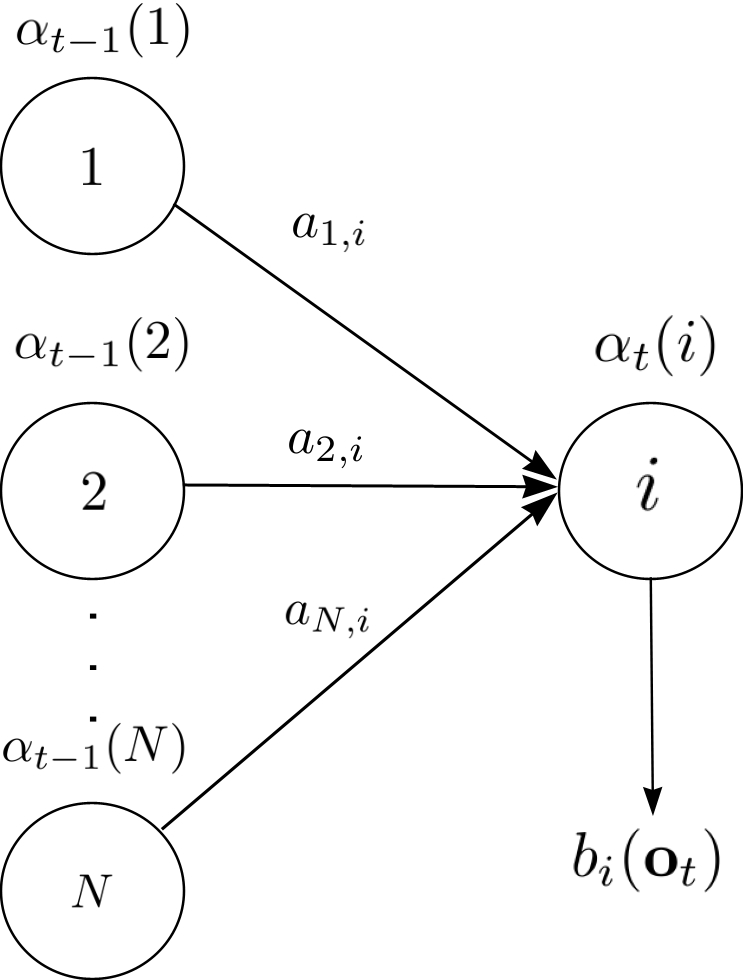
\includegraphics[width=0.25\textwidth]{forward2.jpg}
 \caption{Forward probability}
\end{figure}
The posterior probability of the observation sequence is subsequently calculated by summing over all possible end-states:
\begin{equation}
 P({\bf O}|\lambda) = \displaystyle \sum_{i = 1}^{N} \alpha_{T}(i)
\end{equation}
This holds a complexity of only $\mathcal{O}(N^{2}T)$, which is considerably less than the exponential time. Similarly, a backward probability is defined, which conveys the probability of observing the remaining data in state $i$ at time $t$, $P({\bf o}_{t+1},{\bf o}_{t+2},\ldots, {\bf o}_{T}| q_{t} = s_{j}, \lambda)$ and can be efficiently computed according to:
\begin{equation}
 \label{backwardProbability}
\beta_{t}(i) = \displaystyle \sum_{i=j}^{N} a_{ij} b_{j}({\bf o}_{t+1}) \beta_{j}({\bf o}_{t+1})
\end{equation}
Although we do not need $\beta$ for the computation of $P({\bf O}|\lambda)$, it is provides a comprehensible variable for the training of the model parameters, which  is done by {\it Baum-Welch re-estimation}, a special instance of the EM-algorithm.
\subsection{Baum-Welch re-estimation}
To train the model, we need to maximize the likelihood of the parameters $\mathcal{L}(\lambda|{\bf O})$, by taking partial derivatives of every variable and setting it to zero. If we knew the probability of being in a state at a time step, we could analytically optimize the model parameters and if we knew the model parameters we could estimate the probability of being in a state at a time step. Therefore, we are presented with a chicken-or-egg problem and are left to the mercy of the EM algorithm, which iteratively computes and optimizes these values. For the left-to-right model, the probability of entering state 1, is initialized to 1 and therefore parameter $\pi_{i}$ will remain fixed during the whole re-estimation procedure. To make the rest of the update steps more comprehensible, a set of intermediate variables is defined. First, the probability of begin in a state $i$ at time step $t$, $P(q_{t} = s_{i} | {\bf O}, \lambda )$, which by Bayes' theorem and the before defined forward and backward probabilities can be written as:
\begin{equation}
 \gamma_{t}(i) \equiv (P({\bf O}|\lambda))^{-1} \alpha_{t}(i)\beta_{t}(i) 
\end{equation}
Where normalization constant $P({\bf O}|\lambda) = \sum_{j=1}^{N} \alpha_{t}(i)\beta_{t}(i) = \sum_{j=1}^{N} \alpha_{T}(j)$. To estimate the transition probability between states, we also need the probability of being in a state at $t$ and subsequently transitioning to another state, which is provided by:
\begin{equation}
 \xi_{t}(i,j) \equiv (P({\bf O}|\lambda))^{-1} \alpha_{t}(i)a_{ij}b_{j}({\bf o}_{t})\beta_{t}(j)
\end{equation}
Where $\sum_{j=1}^{N} \xi_{t}(i,j) = \gamma_{t}(i)$. With these variables defined, we can easily and intuitively update the transition function, by marginalizing over all possible time steps:
\begin{equation}
 \hat{a}_{ij} = \frac{ \sum_{t=1}^{T-1} \xi_{t}(i,j) } { \sum_{t=1}^{T-1} \gamma_{t}(i) }
\end{equation}
The update rules for the observation function depend on the distribution used.
\subsection{Observation modeling}
A common choice for an observation function is the Gaussian distribution. However, if we assume one state for every letter, a disadvantage in using a single Gaussian, is that for different writing styles of the same class, the Gaussian model might be trained to give the highest probability for a letter in between two instances. The intuition is illustrated in figure 3, where two different writing styles of an {\it f} are plotted in a two dimensional feature space.
\begin{figure}[ht]
  \centering
  \subfigure[Fit for single Gaussian]{
    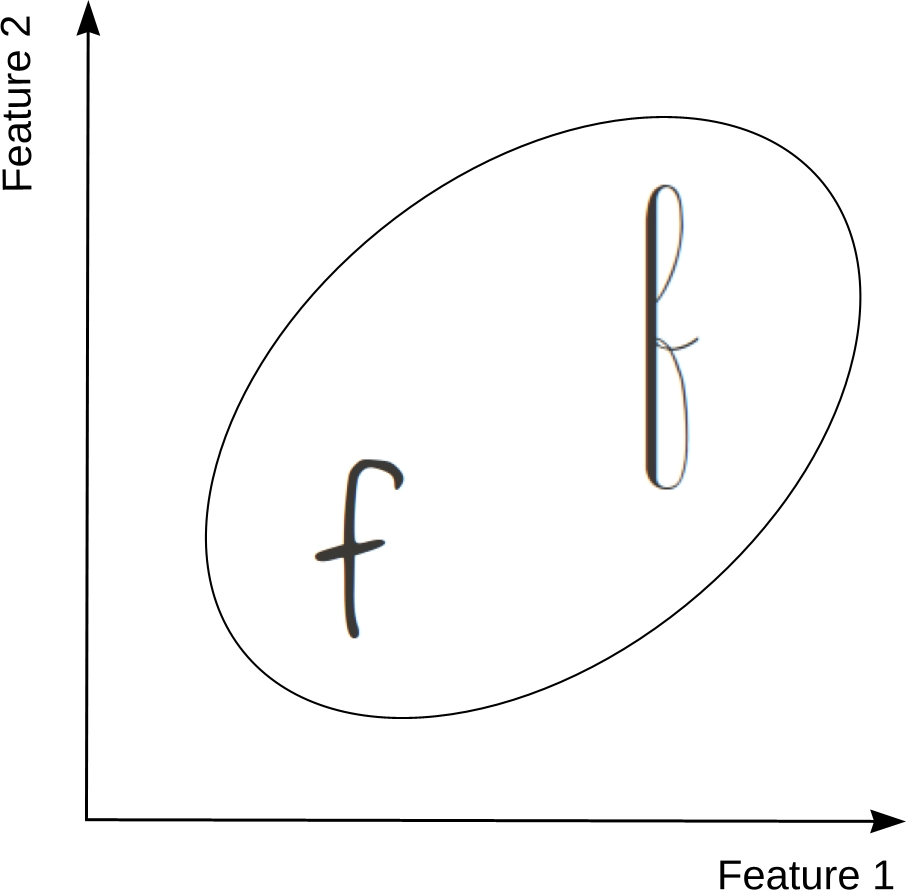
\includegraphics[scale=0.5]{single.jpg}
    \label{fig:subfig1}
  }
  \subfigure[Fit for mixture of Gaussians]{
    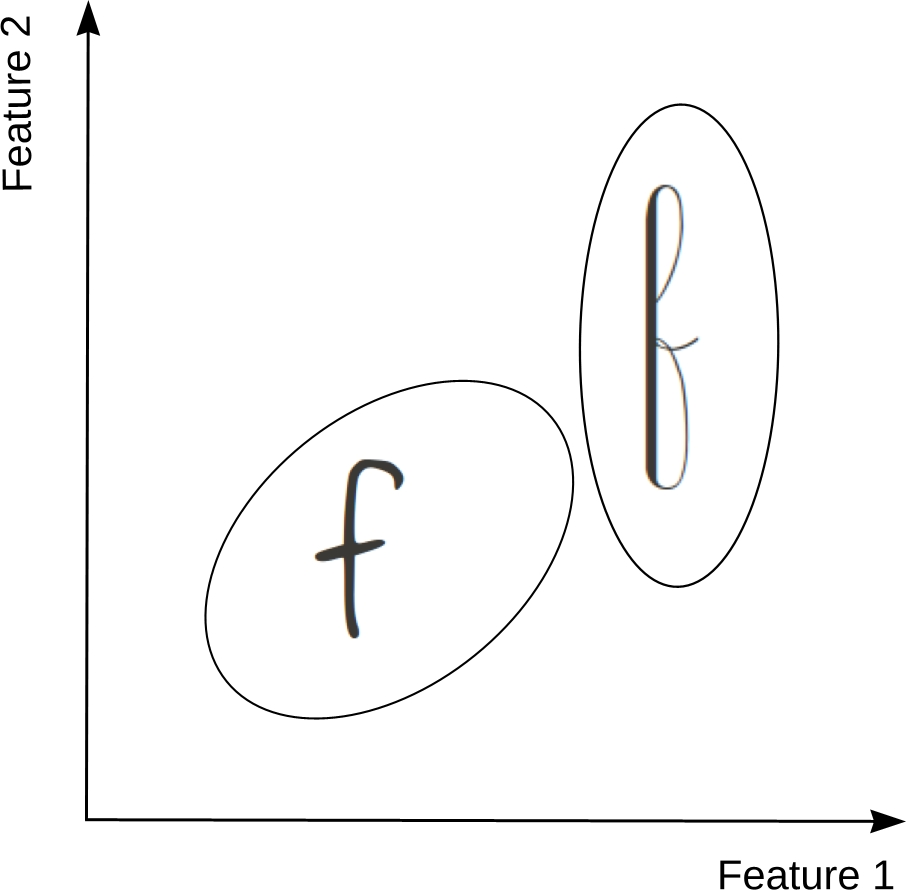
\includegraphics[scale=0.5]{gmm.jpg}
    \label{fig:subfig2}
  }
  \label{fig:subfigureExample}
  \caption[Optional caption for list of figures]{Intuition behind the Gaussian mixture model}
\end{figure}
The Gaussian mixture model (GMM) conveys the following observation function:
\begin{equation}
\label{MOGprobability}
 b_{j}({\bf o}_{t}) = \displaystyle \sum_{k = 1}^K w_{k} \mathcal{N}({\bf o}_{t}; \mu_{jk}, \Sigma_{jk})
\end{equation}
Where $w_{k}$ denotes the prior probability of mixture component $k$, or weight of the mixture. In the case of a GMM, an additional latent variable, the weight of each mixture component, is introduced to the system and we need to adjust the E-step slightly:
\begin{equation}
 \gamma_{t}(i,k) \equiv \gamma_{t}(i) \frac{ b_{i,k}({\bf o}_{t}) } { b_{i}({\bf o}_{t}) }
\end{equation}
The new mixture weights at each iteration are now computed according to:
\begin{equation}
 \label{updateWeightGMM}
 \hat{w}_{i,k} = \displaystyle \frac{\sum_{t=1}^{T} \gamma_{t}(i,k) }{ \sum_{t=1}^{T} \gamma_{t}(i) }
\end{equation}
The new mean is computed by:
\begin{equation}
 \label{updateMeanGMM}
 \hat{\bf{\mu}}_{i,k} = \displaystyle \frac{ \sum_{t=1}^{T} \gamma_{t}(i,k) {\bf o}_{t} }{ \sum_{t=1}^{T} \gamma_{t}(i,k) }
\end{equation}
And the covariance is updated as:
\begin{equation}
 \label{updateCovarianceGMM}
 \hat{\Sigma}_{i,k} = \displaystyle \frac{ \sum_{t=1}^{T} \gamma_{t}(i,k) ({\bf o}_{t} - {\bf \mu}_{i,k})( {\bf o}_{t} - {\bf \mu}_{i,k} )^{T} }{ \sum_{t=1}^{T} \gamma_{t}(i,k) }
\end{equation}
Please note that the update rules for a single Gaussian can easily be derived by setting $K$ to 1. The GMM introduces a scala of additional hyper parameters, such as the number of mixture components and the shape of the covariance matrix. The next section will cover the experimental setup and results acquired with different parameter settings.
\section{Experiments}
The implementation is written in MATLAB due to the flexibility of its Image Processing Toolbox. 
\section{Discussion}
The assumption that a character is stationary over a number of observations may be false. Even though some features like loops output 1, whenever a loop is present in the window, other features do output continuous values and violate this assumption.

-problem of short v long words

\bibliographystyle{plain}
\bibliography{projectAI.bib}

\end{document}
